\part{Dodecahedra: A Model for Alveoli}
\label{partDodecahedron}

Typical alveoli are fourteen sided polyhedra with one face normally being open as a mouth to an alveolar duct \cite{HoppinHildebrandt77}.  To capture the microstructural features of lung, researchers have modeled both alveoli and alveolar ducts, as seen in Fig.~\ref{figRatLung}; we only address alveoli here.  Three different geometric shapes are typically employed when modeling an alveolus: a dodecahedron introduced by Frankus \& Lee \cite{FrankusLee74} in 1974, a rhombic dodecahedron introduced by de~Ryk, Thiesse, Namati \& McLennan \cite{Ryketal07} in 2007, and a truncated octahedron, i.e., a tetrakaidecahedron, introduced by Dale, Matthews \& Schroter \cite{Daleetal80} in 1980.  The dodecahedron and rhombic dodecahedron are both twelve sided polyhedra with faces being pentagons and rhombuses, respectively.  A tetrakaidecahedron is a pair of pyramids stacked bottom to bottom, forming an octahedron, whose six points are then removed.  The end result is a fourteen sided polyhedron with six faces that are squares and eight faces that are hexagons, where like shapes have like dimensions.

The tetrakaidecahedron and rhombic dodecahedron are both volume filling.  This property is preferred whenever one sets out to construct assemblages of alveoli to build a micro\-structural model that is to be solved numerically via a finite element method.  The purpose of such an exercise is to homogenize the response of an alveolar assembly up to the macroscopic level, i.e., the level of a continuum mass point, a.k.a., the parenchyma \cite{Daleetal80,DennySchroter95,DennySchroter97,DennySchroter00,Koweetal86,Ryketal07,Chenetal14}.  Such a finite element model can serve as a representative volume element (RVE) for parenchyma.

The dodecahedron is an isotropic structure, or very nearly so as we shall show, and is nearly volume filling \cite{Kimmeletal87}.  It becomes the preferred geometry whenever a single alveolus is to be used as the RVE of homo\-genization, and from which closed form solutions have been derived \cite{BudianskyKimmel87,KimmelBudiansky90,Kimmeletal87,Freedetal12}.  Here isotropy of the microstructure ensures an isotropic macro response.  Parenchyma, as a tissue, is isotropic \cite{Weedetal15,Fung88,Hughesetal72}; whereas, lung, as an organ, is a complex, heterogeneous structure \cite{Mead73,West07}.  This distinction has, from time-to-time, gotten lost \cite{DennySchroter06}.  

For the reasons stated above, a dodecahedron, with vertices labeled according to Fig.~\ref{figDodecahedron}, is the geometric structure selected for use in this study.
A dodecahedron contains twelve pentagons.  As such, we address the geometry of a pentagon first.  

\begin{figure}
	{\par\centering
		\resizebox*{0.45\textwidth}{0.3\textheight}
		{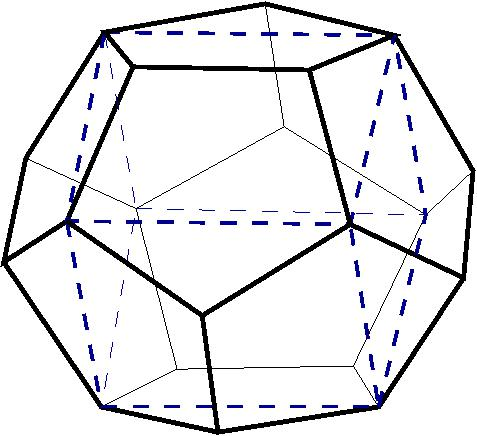
\includegraphics{figures/dodecahedron.jpg}} 
		\resizebox*{0.45\textwidth}{0.3\textheight}
		{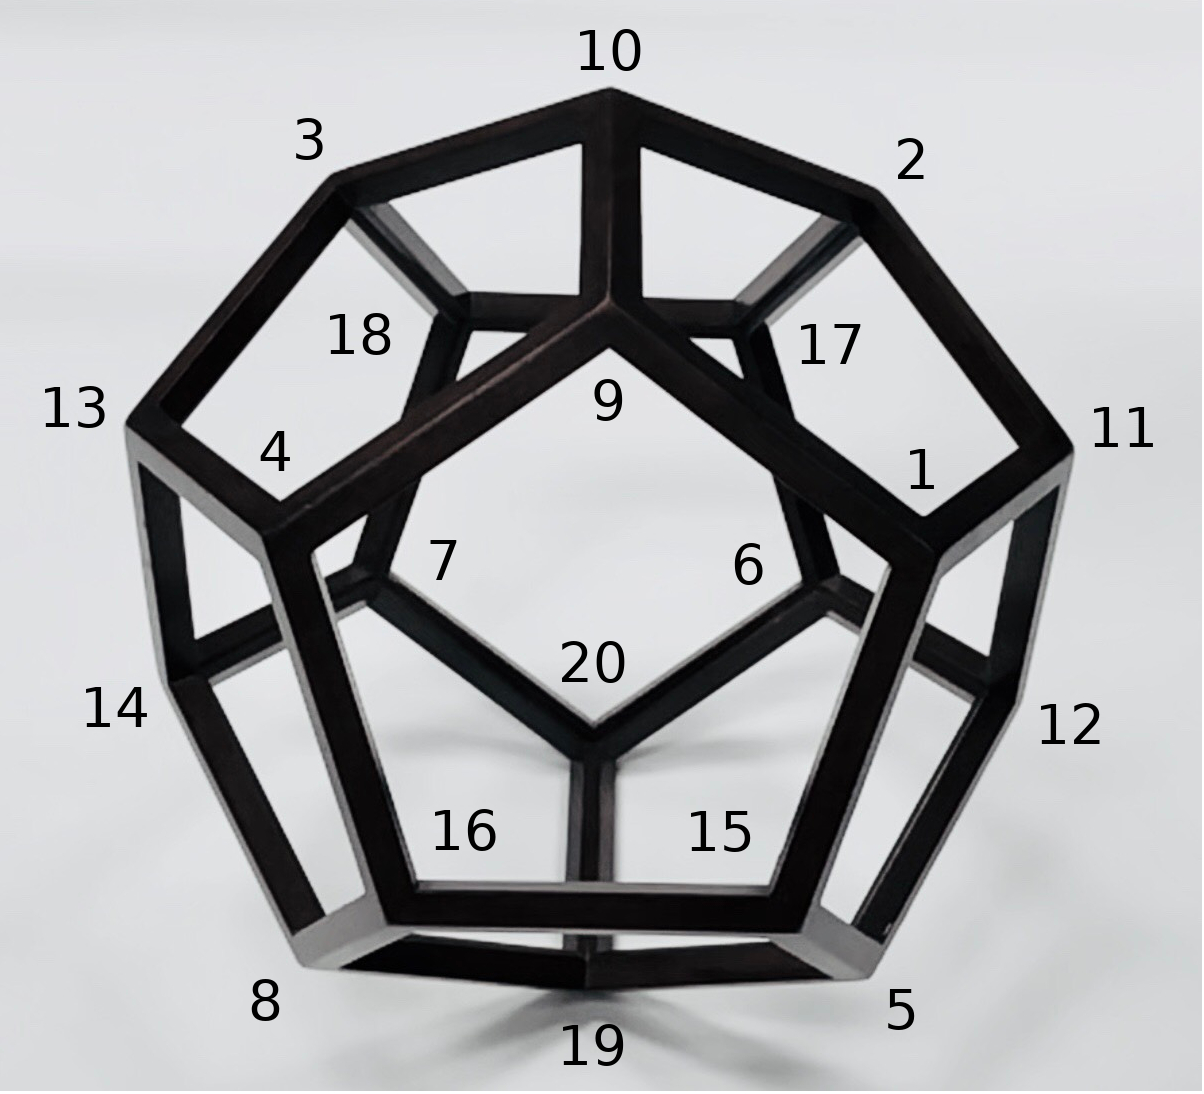
\includegraphics{figures/dodecahedronVertices.jpg}}
		\par}
	\caption{Geometric representations for a dodecahedron.  Left image:  A cube is contained within a dodecahedron, with one of its five possible orientations being displayed.  Atop each face of the cube resides four pentagonal sub-areas that form the shape of a hipped roof line.  Right image:  Vertices 1 through 8 are located at the corners of such a cube.  The centroid for the cube is also the centroid for the dodecahedron.  Vertices 9 through 20 are corners of the hipped roof lines residing above each face of the cube.}
	\label{figDodecahedron}
\end{figure}

\section{Properties of a Regular Pentagon}

Figure~\ref{figRegPentagon} presents a regular pentagon drawn in its natural co-ordinate system with co\-ordinates designated as $(\xi, \eta)$.  Vertices of such a pentagon are placed at
\begin{equation}
	\xi = \cos \left( \frac{2(k-1)\pi}{5} + \frac{\pi}{2} \right) \quad
	\eta = \sin \left( \frac{2(k-1)\pi}{5} + \frac{\pi}{2} \right) \quad
	k = 1, 2, \ldots, 5
	\label{regPentagon}
\end{equation}
wherein $k$ denotes the vertex number, as assigned in Fig.~\ref{figRegPentagon}.  These vertices inscribe a pentagon within the unit circle.

\begin{figure}
	\centering
	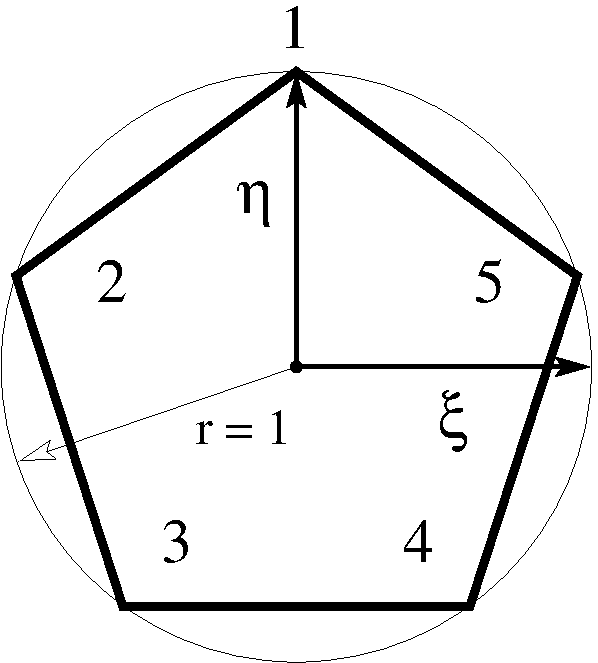
\includegraphics[width=6cm]{figures/regPentagon.pdf}
	\caption{A regular pentagon inscribed within the unit circle establishes its natural co\-ordinate system with co-ordinates $(\xi, \eta)$ described in Eqn.~(\ref{regPentagon}), and whose origin is located at its centroid.  Vertices are numbered counterclockwise with the uppermost vertex being labeled~1.}
	\label{figRegPentagon}
\end{figure}

Lengths of the five chords in a regular pentagon, when measured in its natural co-ordinate system, are all
\begin{equation}
	L^{\!p} = 2 \cos (\omega) \approx 1.176 
	\label{regPentagonLength}
\end{equation}
while the area of this pentagon is
\begin{equation}
	A^p = \tfrac{5}{4} \tan ( \omega ) \, L^{\!p^2} = 
	5 \sin (\omega) \cos (\omega) \approx 2.378
	\label{regPentagonArea}
\end{equation}
where the area of an unit circle is $\pi r^2 \approx 3.142$ because $r=1$.  The
inside angles of a regular pentagon all measure $2\omega = 108^{\circ}$.  All approximations are truncated at four significant figures.

\subsection{Properties of a Regular Dodecahedron}

Like the pentagon considered above, which inscribes the unit circle, here we consider a dodecahedron that inscribes the unit sphere.  Let this geometry be described in its natural co-ordinate system with co-ordinates $(\xi , \eta , \zeta )$ whose origin is located at its centroid, the center of the sphere.  The twenty vertices of this dodecahedron, all of which touch the unit sphere, are placed at
\begin{equation}
\begin{tabular}{ccc}
	$\xi$ & $\eta$ & $\zeta$ \\ \hline
	$\pm 1 / \sqrt{3}$ & $\pm 1 / \sqrt{3}$ & $\pm 1 / \sqrt{3}^{\vphantom{|}}$ \\
	$\pm \phi / \sqrt{3}$ & $\pm 1 / \sqrt{3} \phi$ & 0 \\
	0 & $\pm \phi / \sqrt{3}$ & $\pm 1 / \sqrt{3} \phi$ \\
	$\pm 1 / \sqrt{3} \phi$ & 0 & $\pm \phi / \sqrt{3}$
\end{tabular}
\label{regDodecahedron}
\end{equation}
where $\phi = (1 + \sqrt{5})/2 \approx 1.618$ is also known as the golden ratio.

Lengths of the thirty chords in a regular dodecahedron, when measured in its natural co-ordinate system, are all
\begin{equation}
	L^{\!d} = \frac{2}{\sqrt{3} \phi} \approx 0.7136
	\label{regDodecahedronLength}
\end{equation}
while the volume of such a dodecahedron is
\begin{equation}
	V^d = \frac{40}{3 \sqrt{3} \phi^3} \tan^2 ( \omega ) \sin ( \omega ) \approx 2.785
\label{regDodecahedronVolume}
\end{equation}
where volume of the unit sphere is $\tfrac{4}{3} \pi r^3 \approx 4.189$ because $r=1$.

The scale factor to map between the natural co-ordinates of a pentagon, defined in Eq.~(\ref{regPentagon}), with those of a dodecahedron, defined in Eq.~(\ref{regDodecahedron}), is
\begin{equation}
	\frac{L^{\!p}}{R^p} = \frac{L^{\!d}}{R^p_d} 
	\quad \text{or} \quad
	R^p_d = \frac{R^p L^{\!d}}{L^{\!p}} = \frac{L^{\!d}}{L^{\!p}} = 
	\frac{1}{\sqrt{3} \phi \cos (\omega)} \approx 0.6071
	\label{scaleFactor}
\end{equation}
because $R^p = 1$, with scale factor $R^p_d$ being the radius that inscribes a pentagon on the surface of a dodecaheron that itself inscribes the unit sphere.

\subsection{Dimensions of Human Alveoli}
\label{alveolarSize}

Septal chord length $L(D)$, expressed as a function of alveolar diameter $D$, can be estimated by considering the areal projection of a dodecahedron onto a plane that contains one of its pentagonal faces, which leads to
\begin{equation}
	L = \frac{D}{\tan ( \omega ) ( 1 + \cos ( \alpha ) )} 
	\approx  \frac{D}{2.685} ,
\label{dodecahedralHeight}
\end{equation} 
where $\alpha = \textfrac{\pi}{10} = 18^{\circ}$.  (There are twenty, equal, pie-shaped wedges that comprise this projected area.)  This is an average of the shortest and longest distances across this plane of projection.  Alveolar diameter $D$ is a property that can be measured during an histological study of parenchyma.  

To dimension the alveoli of human lung, Sobin, Fung \& Tremer \cite{Sobinetal88} measured the mean diameter across an individual alveolus, viz., $D$ of Eq.~(\ref{dodecahedralHeight}),  sectioned from human lungs that were fixed at three different pressures.  Samples were taken from nine lungs extracted postmortem from individuals between 16 to 89 years of age.\footnote{%
	Sobin \textit{et~al}.\ \cite{Sobinetal88} documented an age effect in these data that has been averaged over here, i.e., ignored.
}
At a transpulmonary pressure of 4~cm~$\text{H}_2$O, the mean alveolar diameter was $D = 191$ $\pm$ 86~$\mu$m determined from a sampling size of 1423; at a pressure of 10~cm~$\text{H}_2$O, $D = 202$ $\pm$ 88~$\mu$m determined from a sampling size of 1296; and at a pressure of 14~cm~$\text{H}_2$O, $D = 235$ $\pm$ 99~$\mu$m determined from a sampling size of 1083.  These data are plotted in Fig.~\ref{septalLengthFig}.  All reported and drawn error bounds pertain to plus\slash minus one standard deviation in error.  The distribution was found to be normal.

\begin{figure}
	\centering
	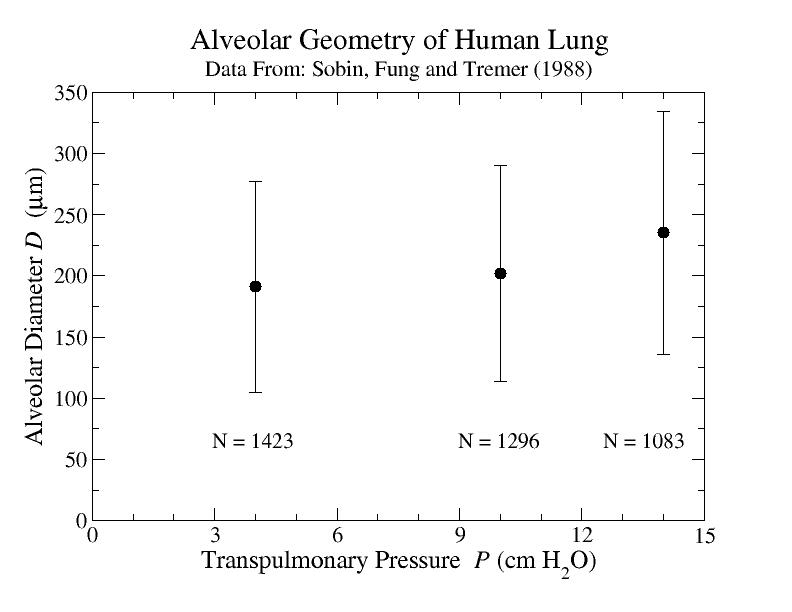
\includegraphics[width=0.4\textwidth]{figures/septalLength.jpg}
    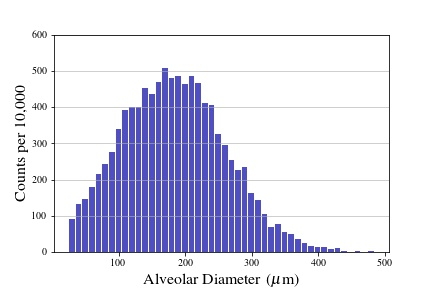
\includegraphics[width=0.44\textwidth]{figures/alveolarDiaHistogram.jpg}
	\caption{Mean and standard deviations for alveolar diameter in human lung illustrated in the left graphic, as reported by Sobin \textit{et~al}.\ \cite{Sobinetal88}, with a typical histogram for these statistics illustrated in the right graphic.  Note that this distribution has been truncated at an alveolar diameter of 24~$\mu$m.}
	\label{septalLengthFig}
\end{figure}

\subsection{Geometries of an Irregular Dodecahedron}
\label{sec:geometries}

Formul\ae\ (\ref{regPentagonArea} \& \ref{regDodecahedronVolume}) only apply for regular pentagons and dodecahedra evaluated in their respective natural co-ordinate systems.  For irregular dodecahedra, the areas of its irregular pentagons are calculated via\footnote{
	Bourke, P., ``Polygons, Meshes.'' \texttt{http://paulbourke.net/geometry}.
}
\begin{equation}
	A = \frac{1}{2} \sum_{i=1}^5 ( x_i y_{i+1} - x_{i+1} y_i)
	\label{irregularPentagonArea}
\end{equation}
where $x_6 \Leftarrow x_1$ and $y_6 \Leftarrow y_1$.  In order for the predicted area to be positive when using this formula, it is necessary that the vertices $(x_i , y_i)$ index counterclockwise, as drawn in Fig.~\ref{figRegPentagon}.  The centroid of this pentagon has co-ordinates\footnotemark[\value{footnote}]
\begin{subequations}
	\label{centroidPentagon}
	\begin{align}
		c_x & = \frac{1}{6 A} \sum_{i=1}^5 (x_i + x_{i+1})
			( x_i y_{i+1} - x_{i+1} y_i) \\
		c_y & = \frac{1}{6 A} \sum_{i=1}^5 (y_i + y_{i+1})
		( x_i y_{i+1} - x_{i+1} y_i)
	\end{align}
\end{subequations}
wherein the vertex co-ordinates $x_i$ and $y_i$ are quantified in a 2D pentagonal frame of reference, e.g., as established later in Fig.~\ref{figPentagonCoord}.

To compute the volume of an irregular dodecahedron, use the formula\footnote{
	Colins, K.~D., ``Cayley-Menger Determinant.'' From MathWorld--A Wolfram Web Resource, created by Eric W.\ Weisstein. \texttt{http://mathworld.wolfram.com/Cayley\-MengerDeterminant.html}.
}
\begin{equation}
	288 V^2_{tet} = \left| \begin{matrix}
	0 & 1 & 1 & 1 & 1 \\
	1 & 0 & \ell_{12}^{\,2} & \ell_{13}^{\,2} & \ell_{14}^{\,2} \\
	1 & \ell_{21}^{\,2} & 0 & \ell_{23}^{\,2} & \ell_{24}^{\,2} \\
	1 & \ell_{31}^{\,2} & \ell_{32}^{\,2} & 0 & \ell_{34}^{\,2} \\
	1 & \ell_{41}^{\,2} & \ell_{42}^{\,2} & \ell_{43}^{\,2} & 0
	\end{matrix} \right|
	\label{tetrahedralVolume}
\end{equation}
to calculate each of the 60 individual tetrahedral volumes that collectively fill the volume of an irregular dodecahedron.  Here $\ell_{ij}$ is the length of that tetrahedral edge with vertices $i$ and $j$; $i, j = 1, 2, 3, 4$; $i \neq j$; with $\ell_{ij} = \ell_{ji}$.

\subsection{Indexing Scheme for Dodecahedra}

In order to implement the dodecahedron as a geometric model for an alveolar sac, as suggested by the images in Fig.~\ref{figRatLung}, it first becomes necessary to introduce a labeling strategy. Such a scheme is arbitrary, but once chosen it enables an analysis to be put forward.  The labeling scheme adopted in this work is illustrated in the right image of Fig.~\ref{figDodecahedron}. 
  
The co-ordinates positioning the twenty vertices of a regular dodecahedron in its natural frame of reference are presented in Table~\ref{TableDodecahedron}.  According to the labeling scheme of Fig.~\ref{figDodecahedron}, the thirty chords of a dodecahedron are given vertex assignments according to Table~\ref{Tablechordae}, while its twelve pentagons are given vertex assignments according to Table~\ref{TablePentagons}.

\begin{table}
	\begin{center}
	\begin{tabular}{|c|ccc||c|ccc|}
		\hline 
		Vertex & $\xi$ & $\eta$ & $\zeta$ & Vertex & $\xi$ & $\eta$ & $\zeta$ \\ \hline
		1 & $1 / \sqrt{3}$ & $1 / \sqrt{3}$ & $1 / \sqrt{3}^{\vphantom{|}}$ & 
		   11 & $\phi / \sqrt{3}$ & $1 / \sqrt{3} \phi$ & 0 \\
		2 & $1 / \sqrt{3}$ & $1 / \sqrt{3}$ & -$1 / \sqrt{3}$ & 
		   12 & $\phi / \sqrt{3}$ & -$1 / \sqrt{3}\phi$ & 0 \\
		3 & -$1 / \sqrt{3}$ & $1 / \sqrt{3}$ & -$1 / \sqrt{3}$ & 
		   13 & -$\phi / \sqrt{3}$ & $1/ \sqrt{3}\phi$ & 0 \\
		4 & -$1 / \sqrt{3}$ & $1 / \sqrt{3}$ & $1 / \sqrt{3}$ & 
		   14 & -$\phi / \sqrt{3}$ & -$1 / \sqrt{3}\phi$ & 0 \\
		5 & $1 / \sqrt{3}$ & -$1 / \sqrt{3}$ & $1 / \sqrt{3}$ & 
		   15 & $1 / \sqrt{3} \phi$ & 0 & $\phi / \sqrt{3}$ \\
		6 & $1 / \sqrt{3}$ & -$1 / \sqrt{3}$ & -$1 / \sqrt{3}$ & 
		   16 & -$1 / \sqrt{3}\phi$ & 0 & $\phi / \sqrt{3}$ \\
		7 & -$1 / \sqrt{3}$ & -$1 / \sqrt{3}$ & -$1 / \sqrt{3}$ & 
		   17 & $1 / \sqrt{3}\phi$ & 0 & -$\phi / \sqrt{3}$ \\
		8 & -$1 / \sqrt{3}$ & -$1 / \sqrt{3}$ & $1 / \sqrt{3}$ & 
		   18 & -$1 / \sqrt{3}\phi$ & 0 & -$\phi / \sqrt{3}$ \\
		9 & 0 & $\phi / \sqrt{3}$ & $1 / \sqrt{3}\phi$ & 
		   19 & 0 & -$\phi / \sqrt{3}$ & $1 / \sqrt{3}\phi$ \\
		10 & 0 & $\phi / \sqrt{3}$ & -$1 / \sqrt{3}\phi$ & 
		   20 & 0 & -$\phi / \sqrt{3}$ & -$1 / \sqrt{3}\phi$ \\
		\hline
	\end{tabular}
	\end{center}
	\caption{Natural co-ordinates for the vertices of a regular dodecahedron, as labeled in Fig.~\ref{figDodecahedron} according to Eq.~(\ref{regDodecahedron}).}
	\label{TableDodecahedron}
\end{table}

The sixty tetrahedra that fill the volume of the dodecahedron contain vertices according to the following strategy.  Beginning with pentagon~1 and sequencing to pentagon~12, two of the four vertices come from a side of the pentagon in question with the remaining two vertices being the centroid for that pentagon and the centroid of the, i.e., at the coordinate origin.  From Table~\ref{TablePentagons}, tetrahedron~1 contains vertices 11 and 2 of pentagon~1, tetrahedron~2 contains vertices 2 and 10, tetrahedron~3 contains vertices 10 and 9, tetrahedron~4 contains vertices 9 and 1, tetrahedron~5 contains vertices 1 and 11, tetrahedron~6 contains vertices 10 and 2 from pentagon~2, etc.

\begin{table}
	\begin{center}
	\begin{tabular}{|c|c||c|c||c|c|}
		\hline
		Chord & Vertices & Chord & Vertices & Chord & Vertices \\ \hline
		1 & 9, 10 & 11 & 17, 18 & 21 & 7, 18 \\
		2 & 1, 9 & 12 & 3, 18 & 22 & 7, 14 \\
		3 & 2, 10 & 13 & 4, 16 & 23 & 13, 14 \\
		4 & 3, 10 & 14 & 15, 16 & 24 & 8, 14 \\
		5 & 4, 9 & 15 & 1, 15 & 25 & 8, 16 \\
		6 & 1, 11 & 16 & 5, 15 & 26 & 5, 19 \\
		7 & 2, 11 & 17 & 5, 12 & 27 & 6, 20 \\
		8 & 3, 13 & 18 & 11, 12 & 28 & 7, 20 \\
		9 & 4, 13 & 19 & 6, 12 & 29 & 8, 19 \\
		10 & 2, 17 & 20 & 6, 17 & 30 & 19, 20 \\
		\hline
	\end{tabular}
	\end{center}
	\caption{Vertices that locate the endpoints of septal chords in a dodecahedron, as labeled in Fig.~\ref{figDodecahedron}.}
	\label{Tablechordae}
\end{table}

\begin{table}
	\begin{center}
	\begin{tabular}{|c|c|c|}
		\hline
		Pentagon & Vertices & Chords \\ \hline
		1 & 11, 2, 10, 9, 1 & 6, 7, 3, 1, 2 \\
		2 & 10, 2, 17, 18, 3 & 4, 3, 10, 11, 12 \\
		3 & 13, 4, 9, 10, 3 & 8, 9, 5, 1, 4 \\
		4 & 9, 4, 16, 15, 1 & 2, 5, 13, 14, 15 \\
		5 & 15, 5, 12, 11, 1 & 15, 16, 17, 18, 6 \\
		6 & 17, 2, 11, 12, 6 & 20, 10, 7, 18, 19 \\
		7 & 18, 7, 14, 13, 3 & 12, 21, 22, 23, 8 \\
		8 & 16, 4, 13, 14, 8 & 25, 13, 9, 23, 24 \\
		9 & 12, 5, 19, 20, 6 & 19, 17, 26, 30, 27 \\
		10 & 14, 7, 20, 19, 8 & 24, 22, 28, 30, 29 \\
		11 & 20, 7, 18, 17, 6 & 27, 28, 21, 11, 20 \\
		12 & 19, 5, 15, 16, 8 & 29, 26, 16, 14, 25 \\
		\hline
	\end{tabular}
	\end{center}
	\caption{Vertices that locate the corners of regular pentagonal surfaces in a regular dodecahedron, and the chords that connect them.  They are indexed counterclockwise when viewed looking from the outside in, and labeled according to Fig.~\ref{figDodecahedron}.  The apex for each pentagon resides at the peak of the hipped roof-line for that pentagon.  This turns out to be important.} 
	\label{TablePentagons}
\end{table}

\subsection{Co-ordinate Systems for Chordal Fibers and Pentagonal Membranes}

The dodecahedron used to model an alveolus is considered to be regular in its `natural' configuration, with the capability of being irregular in its reference configuration, and certainly becoming irregular when deformed.  The co-ordinate frame of this natural state is taken to have its origin positioned at the centroid of this regular dodecahedron, i.e., at the centroid of an enclosed cube (cf.\ Fig.~\ref{figDodecahedron}) or, equivalently, at the origin of the unit sphere they inscribe, as presented in Table~\ref{TableDodecahedron}.  We denote the base vectors associated with this frame of reference as $( \vec{\boldsymbol{\imath}} , \vec{\boldsymbol{\jmath}} , \vec{\mathbfit{k}} \, )$.  There are two other co-ordinate systems with relevance to our analysis: those for the chordal fibers, and those for the pentagonal membranes.

The local co-ordinate system of a chordal fiber is presented in Fig.~\ref{figchord}, while the local co-ordinate system of a pentagonal membrane is presented in Fig.~\ref{figPentagonCoord}.  The software described in \ref{appchords} and \ref{appPentagons} utilize these co-ordinate systems, whose origins are located at their centroids, along with their rotation and spin matrices, which are measured relative to the co-ordinate frame of the dodecahedron, i.e., relative to $( \vec{\boldsymbol{\imath}} , \vec{\boldsymbol{\jmath}} , \vec{\mathbfit{k}} \, )$.

\begin{figure}
    \centering
    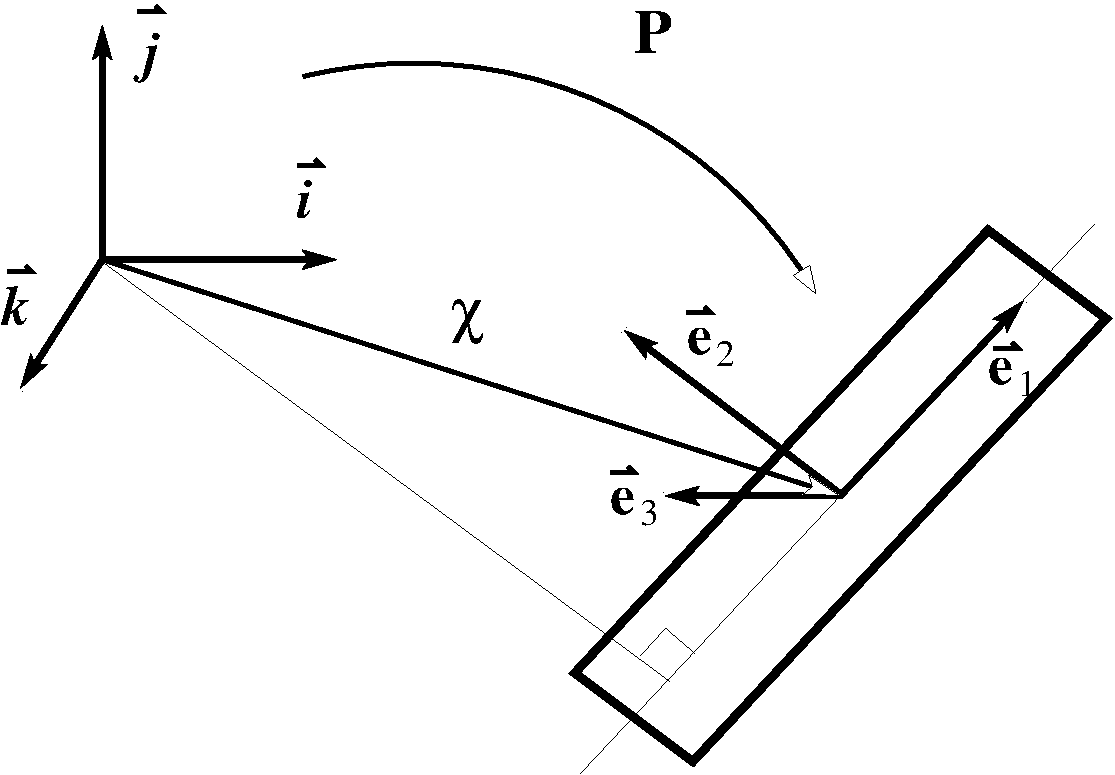
\includegraphics[width=8cm]{figures/chord.pdf}
    \caption{The co-ordinate system of a chord $( \vec{\mathbf{e}}_{\,1} , \vec{\mathbf{e}}_{\,2} , \vec{\mathbf{e}}_{\,3} )$ relative to the co-ordinate system of its dodecahedron $( \vec{\boldsymbol{\imath}} , \vec{\boldsymbol{\jmath}} , \vec{\mathbfit{k}} \,)$ with origins located at their respective centroids that are offset by a translation $\boldsymbol{\chi}$.  These describe a mapping $[ \{ \vec{\mathbf{e}}_{\,1} \} \{ \vec{\mathbf{e}}_{\,2} \} \{ \vec{\mathbf{e}}_{\,3} \} ] = [ \{ \vec{\boldsymbol{\imath}} \, \}\{ \vec{\boldsymbol{\jmath}} \, \}\{ \vec{\mathbfit{k}} \, \} ] \mathbfsf{P}$ where $\mathbfsf{P}$ is an orthogonal rotation.  The tangent base vector $\vec{\mathbf{e}}_{\,1}$ aligns with the axis of this chord. The normal base vector $\vec{\mathbf{e}}_{\,2}$ is coaxial with a line segment drawn from the origin out to the chordal axis such that $\vec{\mathbf{e}}_{\,1} \cdot \vec{\mathbf{e}}_{\,2} = 0$. While the binormal base vector is given by the cross product $\vec{\mathbf{e}}_{\,3} = \vec{\mathbf{e}}_{\,1} \times \vec{\mathbf{e}}_{\,2}$.}
    \label{figchord}
\end{figure}

\begin{figure}
    \centering
    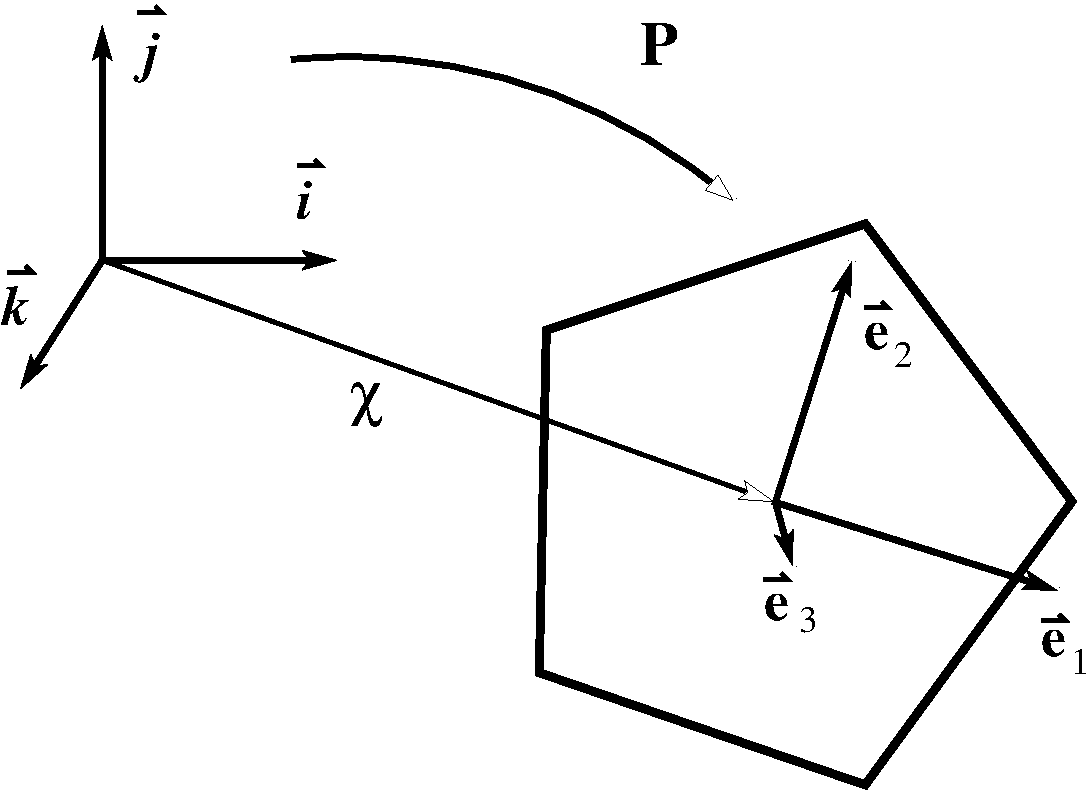
\includegraphics[width=8cm]{figures/pentagonCoord.pdf}
    \caption{The co-ordinate system of a pentagon $( \vec{\mathbf{e}}_{\,1} , \vec{\mathbf{e}}_{\,2} , \vec{\mathbf{e}}_{\,3} )$ relative to the co-ordinate system of its dodecahedron $( \vec{\boldsymbol{\imath}} , \vec{\boldsymbol{\jmath}} , \vec{\mathbfit{k}} \,)$ with origins located at their respective centroids that are offset by a translation $\boldsymbol{\chi}$.  These describe a mapping $[ \{ \vec{\mathbf{e}}_{\,1} \} \{ \vec{\mathbf{e}}_{\,2} \} \{ \vec{\mathbf{e}}_{\,3} \} ] = [ \{ \vec{\boldsymbol{\imath}} \, \}\{ \vec{\boldsymbol{\jmath}} \, \}\{ \vec{\mathbfit{k}} \, \} ] \mathbfsf{P}$ where $\mathbfsf{P}$ is an orthogonal rotation.  Base vector $\vec{\mathbf{e}}_{\,1}$ is coaxial to a line segment that connects two vertices which locate a pair of shoulders in a pentagon, viz., vertices 2 and 5 in Fig.~\ref{figRegPentagon}.  Base vector $\vec{\mathbf{e}}_{\,2}$ is coaxial with a line segment drawn from the head of this pentagon, i.e., vertex 1 in Fig.~\ref{figRegPentagon}, down to its base such that $\vec{\mathbf{e}}_{\,1} \cdot \vec{\mathbf{e}}_{\,2} = 0$.  Base vector $\vec{\mathbf{e}}_{\,3} = \vec{\mathbf{e}}_{\,1} \times \vec{\mathbf{e}}_{\,2}$ is the outward normal to this surface.}
    \label{figPentagonCoord}
\end{figure}

